\paragraph{Frequency Shift Keying:}
Frequency Shift Keying (FSK) is a scheme to transmit digital 
information across an analog channel.  Binary data bits are 
grouped into blocks of a fixed size, and each block is 
represented by a unique carrier frequency, called a symbol, 
to be sent across the channel.  
(The receiver then looks at the recovered symbol frequency to 
determine which block of bits was sent and converts it 
back to the appropriate binary data.)  This requires having 
a unique symbol for each possible combination of 
data bits in a block.  
In this laboratory exercise each symbol 
represents a two-bit block; therefore, there will be four 
different symbols.

The carrier frequency is kept constant over some 
number of samples known as the symbol period ($T_{symb}$).  
The symbol rate, defined as $F_{symb}$, is a fraction of the 
board's sampling rate, $F_s$.  For our sampling rate of 44.1 kHz 
and a symbol period of 32, the symbol rate is 44.1k/32 symbols per second.

\begin{figure}[htb]
   \begin{center}
      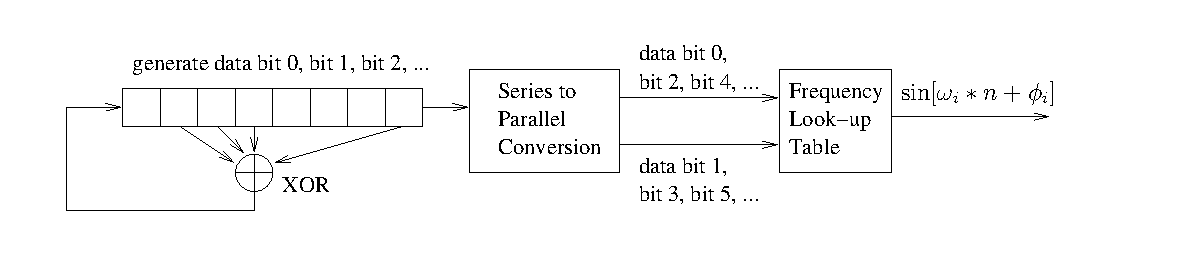
\epsfig{file=trans.eps,width=18cm}
        \caption{Pseudo-noise sequence generator and FSK transmitter.}
      \label{fig:trans}
   \end{center}
\end{figure}

\paragraph{Pseudo-Noise Sequence Generator:}
The input bits to the transmitter are provided by the special 
shift-register, called a pseudo-noise sequence generator 
(PN generator), on the left side of Figure~\ref{fig:trans}.  
A PN generator produces a
sequence of bits that appears random.  The PN sequence will
repeat with period $2^B-1$, where $B$ is the width in bits 
of the shift register.  A more detailed diagram of the PN 
generator alone appears in Figure~\ref{fig:pn-gen}.

\begin{figure}[htb]
   \begin{center}
      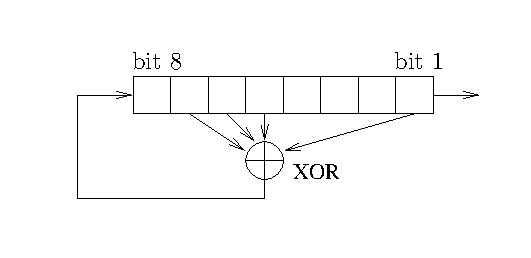
\epsfig{file=pn-gen.eps,width=9cm}
        \caption{PN generator.}
      \label{fig:pn-gen}
   \end{center}
\end{figure}

As shown in Figure~\ref{fig:pn-gen}, the PN generator is simply a
shift-register and XOR gate.  Bits 1, 5, 6, and 7 of the
shift-register are XORed together and the result is shifted
into the highest bit of the register.  The lowest bit, which
is shifted out, is the output of the PN generator.

The PN generator is a useful source of random data bits for
system testing.  We can simulate the bit sequence that would
be transmitted by a user as the random bits generated by the
PN generator.  Since communication systems tend to randomize
the bits seen by the transmission scheme so that bandwidth
can be efficiently utilized, the PN generator is a good data
model.  (PN generators have other applications in communications,
notably in the Code Division Multiple Access schemes used 
by cellular telephones.)

\paragraph{Series-to-Parallel Conversion:} 
The shift-register produces one output bit at a time.  Because each 
symbol the system transmits will encode two bits, we require the 
series-to-parallel conversion to group the output bits from 
the shift-register into blocks of two bits so that they can be mapped 
to a symbol. 

\paragraph{Frequency Look-up Table:} 
This is responsible for mapping blocks of bits to one 
of four frequencies as shown in Figure \ref{fig:trans}. Each 
possible two-bit block of data from the series-to-parallel conversion 
is mapped to a different carrier frequency $\omega_i$.\footnote{Note 
that the subscript $i$ denotes a symbol's index in the transmitted signal; 
i.e., the first symbol sent has index $i=1$, the second symbol sent has 
index $i=2$, and so on.  Therefore, $\omega_i$ denotes the frequency and 
$\phi_i$ denotes the phase offset of the $i$th transmitted symbol.} These 
frequencies are then used to generate the waveforms.  The mappings for 
this assignment are given in the table below.

\begin{tabular}{|r|r|} 
\hline
Data Chunk & Carrier Frequency $\omega_i$\\ \hline\hline
00 & $9\pi/32$\\ \hline 
01 & $13\pi/32$\\ \hline 
11 & $17\pi/32$\\ \hline 
10 & $21\pi/32$\label{table}\\ \hline 
\end{tabular}

One way to implement this mapping is by using a look-up table.  
The two-bit data block can be interpreted as an offset into a 
frequency table where we have stored the possible transmission 
frequencies.  Note that since each frequency mapping defines a 
symbol, this mapping is done at the symbol rate $F_{symb}$, or once 
for every $T_{symb}$ DSP samples.

The symbol bit assignments are such that
any two adjacent frequencies map to data blocks that differ by 
only one bit.  This assignment is called Gray coding and 
helps reduce the number of bit errors made in the event of a 
received symbol error.

\paragraph{Phase Continuity:}
In order to minimize the bandwidth used by the transmitted signal, 
you should ensure that the phase of your transmitted waveform is 
continuous between symbols; i.e., the beginning phase of any symbol 
must be equal to the ending phase of the previous symbol.
For instance, if a symbol of frequency $9\pi/32$ begins at 
phase 0, the symbol will end 31 output samples later
at phase $31*9\pi/32$.  To preserve phase continuity, the next 
output sample must be at phase $32*9\pi/32$, which is 
equivalent to phase $\pi$.  Therefore, the next symbol, 
whatever its frequency, must begin at phase $\pi$.  For each symbol, 
you must choose $\phi_i$ in the expression 
$\sin[\omega_i * n + \phi_i]$ to create this continuity.


